\documentclass[10pt,a4paper]{article}
\usepackage[a4paper,
            left=1in,right=1in,top=1in,bottom=1in,%
            footskip=.25in]{geometry}
\usepackage[latin1]{inputenc}
\usepackage[T1]{fontenc}
\usepackage{amsmath}
\usepackage{amsfonts}
\usepackage{amssymb}
\usepackage{bbm}
\usepackage{multirow}
\usepackage[titletoc, title]{appendix}
\usepackage{float}
%color definitions
\usepackage{color}
\newcommand{\blue}[1]{{\color{blue} #1}}  
\newcommand{\red}[1]{{\color{red} #1}}
%figure definitions to read .eps files from network drives
\usepackage{grffile}
\usepackage{graphicx}
\graphicspath{{Figures/}}
\usepackage{epstopdf}
\usepackage[caption=false]{subfig}
%bibilography definitions to manage special characters and urls
\usepackage{url}
\usepackage{natbib}
 \bibpunct[, ]{(}{)}{,}{a}{}{,}%
 \def\bibfont{\small}%
 \def\bibsep{\smallskipamount}%
 \def\bibhang{24pt}%
 \def\newblock{\ }%
 \def\BIBand{and}%
%to take care of \hbox badness errors
\usepackage{etoolbox}
\apptocmd{\sloppy}{\hbadness 10000\relax}{}{}

% Keywords command
\providecommand{\keywords}[1]
{
  \small	
  \textbf{\textit{Keywords---}} #1
}

\author{Amir A. Nasrollahzadeh, Ardalan Raisi Sofi, Bahram Ravani}
\title{Factors Contributing to Roadside Work Zone Collisions}
\begin{document}
\maketitle
\begin{abstract}\label{se:abs}
Identifying factors that contribute to the probability of roadside work zone collisions enables decision makers to assess and control the risk of scheduling a particular maintenance or construction activity by modifying the characteristics of the operation. This can be achieved by studying the effect of work zone properties on the risk  of roadside work zone collisions. Much of the existing work in this area is based on data in the police traffic collision reports which do not include data on the characteristics of the work zone itself. This paper develops a comprehensive data set of 42 features describing time, location, work zone characteristics, traffic volume, and road properties. This extensive set of features allows for more accurate analysis deriving the effect of each feature on the risk  of work zone collisions. Our statistical analysis reveals 10 important features and shows that four of these features are the most significant in influencing collision risk for a work zone. 
\end{abstract}

\keywords{Work zone collisions, work zone safety, collision risk factors, collision severity, logistic regression, extreme gradient boosting, feature selection}

\section{Introduction}\label{se:intro}
Roadside work zone fatalities have increased by 29\% in the U.S. since 2010 \citep{injuryfacts2020}. This has been despite various public awareness campaigns and multiple training programs in each state rising the level of public awareness about roadside work zone safety. According to the National Highway Traffic Safety Administration (NHTSA), the number of roadside work zone fatalities in California has increased from 42 in 2010 to 65 in 2018, reaching a peak of 75 fatalities in 2016 \citep{caworkfatalities2018}. Moreover, the Bureau of Labor Statistics reports that the number of work zone worker fatalities in California has not declined in the last decade \citep{caworkerfatalities2018}. These historical trends for California are depicted in Figure \ref{fig:fatalities}.

\begin{figure}[hb!]
	\centering
	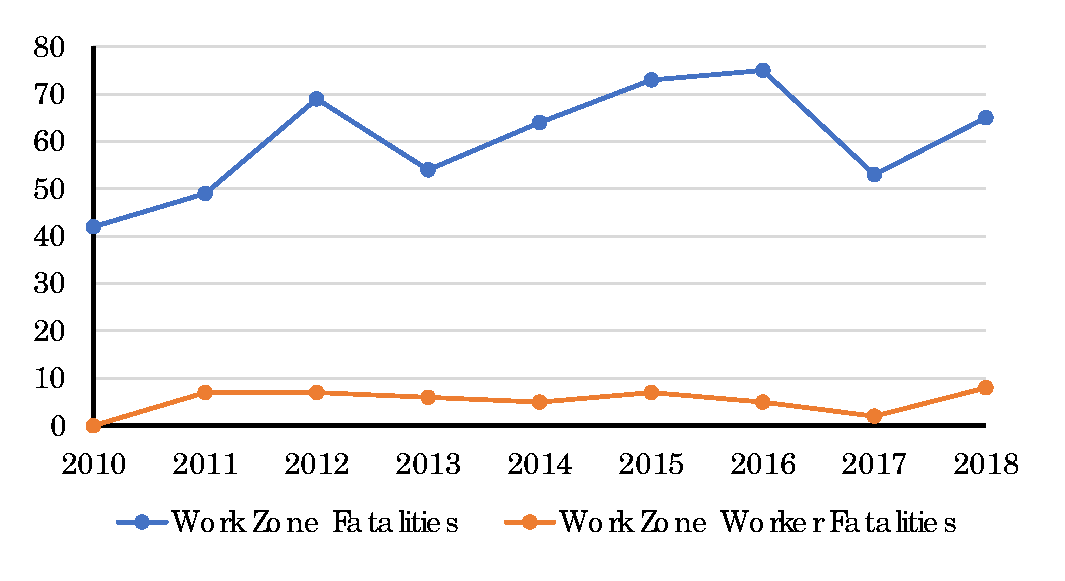
\includegraphics[width=8cm,height=5cm, trim=2cm 10cm 2cm 11cm, clip=true]{WZ fatalities}
	\caption{California work zone fatalities.}
	\label{fig:fatalities}
\end{figure}

Roadside work zones may alter the road geometry, affect the traffic flow and volumes, and change the driving conditions by, for example, limiting visibility or lane closures causing sudden congested traffic. These changes introduce unexpected and incidental circumstances that may increase the probability of motor vehicle collisions resulting in injuries or fatalities. The increasing need to maintain and repair the aging U.S.  highways and road system will require more roadside maintenance activities in the future. In fact, as of 2018, only 59\% of California roads were classified as `acceptable` according to the International Roughness Index \citep{roadcondition2018}. Therefore, studying the factors that contribute to the probability and severity of roadside work zone collisions is justified due to the increasing number of injuries and fatalities at roadside work zones.

Recently, various statistical analysis methods have been adapted to identify factors that contribute to different types and classes of work zone accidents (e.g., rear-end collisions or collisions with fixed objects). However, in most of these studies, the scope of the investigation has been limited by the availability of data describing the work zones or the corresponding collisions. This is partly due to the large variability in the types of information collected for work zone collisions in each state \citep{wzguidline2017}. In addition, most if not all of these studies rely on police collision reports, and although some describe environmental features of an accident (for example, road surface condition, lighting, and weather), they do not report the characteristics of the work zone associated with the collision such as work length, duration, its lane closure features, type of maintenance activity, etc.

In this work, multiple data sets for California Highways from the California Department of Transportation (Caltrans) are utilized, and matched with police collision reports not only capturing data in the police collision reports but also data describing the specifics of a work zone, maintenance activity, and lane closure characteristics. Therefore, the effects of particular maintenance activity and characteristics of its work zone are also captured. Furthermore, traffic volume data, road features, and lane closure information are matched with maintenance work orders allowing construction of a comprehensive data set with 42 features that can be statistically analyzed to identify major factors contributing to the probability and severity of work zone collisions. To the best of our knowledge, this is the first study that considers a comprehensive set of 42 relevant features which are described in more detail in Section \ref{se:data}.

\subsection{Paper Organization}
Section \ref{se:background} reviews the literature related to analyzing work zone collisions. Section \ref{se:data} describes various data sources and their relevant features and the challenges they present. In Section \ref{se:method}, the feature selection method and the logistic regression model used to identify the major factors contributing to the probability %and severity 
of collisions for each roadside work order is presented. Section \ref{se:results} presents the result of numerical analyses, Section \ref{se:discuss} discusses the limitations and potential extensions of this study, and Section \ref{se:conclusion} discusses the conclusion of the paper.

\section{Background} \label{se:background}
The literature review in this section is limited to the descriptive analysis of roadside work zone collisions. It must be noted that there is also an extensive stream of literature that studies the roadside work zone design and examines standards, policies, and costs of planning and scheduling roadside maintenance or construction work orders. These studies are not directly related to the scope of this paper and are not included in the literature review.

%we may want to consider taking the two paragprahs out from this paper and keep it for the severity paper
%A significant portion of relevant studies are focused on comparing work zone collisions with non-work zone crashes. A state-of-the-art review of these studies considered 27 articles from 1962 to 2013 that directly or indirectly compared work zone crashes with non-work zone collisions and concluded that no clear evidence emerges to suggest that work zone collisions are more severe or vice versa \citep{yang2015work}. For example, \cite{ha1995detailed} investigated the severity of collisions in Ohio from 1982 to 1986 and concluded that there is no significant difference between the severity of the work zone and non-work zone collisions. However, Ha and Nemeth's results are in contrast to the results reported by \cite{daniel2000analysis}, which studied the most severe crashes in Georgia from 1995 to 1997 and determined that there is a significant difference between the work zone and non-work zone fatal crashes. Therefore, the literature is undecided on whether the presence of work zones contributes to the severity of crashes; refer to \cite{yang2015work} and references therein for more details. This inconsistency might be due to the limitations of the databases that were investigated since almost all of them were limited to police collision reports, which usually do not include any information about the characteristics of a work zone. In our study, multiple databases are sourced to augment police collision reports with additional features describing work zones, roads, and lane closures.

%Another approach reported in the literature excludes non-work zone collisions and only considers work zone crashes to identify factors that increase the severity of motor vehicles involved in crashes. This is the approach adopted by \cite{wong2011factors}, which identified activity type (on foot worker or driving) and location of the accident (freeway/highway, moving and stationary lane closures) as having the most effect on the severity of work zone collisions. Note that \cite{wong2011factors} utilized the California Crash Injury Database, which recorded work zone accidents explicitly until 2007. The data preparation effort (Section \ref{se:data}) in our study is aimed to replicate such a data set where each roadside work order is described by its features, e.g., work length, closure type, etc., and is then matched to the corresponding police collision report. However, some features of this study, such as whether workers were given personal protective equipment, could not be determined in our study.
% the above two paragraphs most discuss severity and we can cut them out for this paper%

A significant portion of studies analyzing factors that contribute to frequency of work zone collisions are focused on comparing work zone collisions with non-work zone crashes. A state-of-the-art review of these studies considered 21 articles from 1962 to 2013 that directly or indirectly compared work zone crashes with non-work zone collisions and showed that the rate of accidents generally increases in the presence of work zones \citep{yang2015work}. The majority of these studies used negative binomial models to analyze crash frequency because the objective was to predict the number of crashes in a specific period (e.g., duration of work zone) for a particular section of road (e.g., length of work zone); see, for example, \cite{ozturk2013crash} and \cite{yang2013modeling}. \cite{harb2008freeway} compared work zone crashes and non-work zone collisions using the Florida Traffic Crash Records Database for the years 2002 to 2004. This study used various logistic regression models and determined that several factors such as lighting, weather, and truck traffic volumes are more likely to contribute to a work zone collision compared to non-work zone crashes. However, these studies, regardless of the statistical method used, can be susceptible to non-homogeneity errors since they are usually based on a comparison of work zone crashes and non-work zone collisions. This is due to the effect of the work zone on certain types of variables under consideration. For example, one could argue that traffic volume and average speed reduces in the presence of a work zone. However, the data for these features are typically available only for non-work zone situations. Thus, the model will be erroneous when considering such a feature for both work zone and non-work zone crashes. \cite{harb2008freeway} tried to overcome this issue by stratified sampling based on, for example, speed limits such that the crashes in each sub-samples are supported by the same speed distribution. This method is less effective when the number of variables for stratification increases, which leads to smaller sub-samples and less accurate regression analyses. Moreover, its implementation is dependent on the availability of data for both the work zone and non-work zone crashes, which is rarely the case, as \cite{yang2015work} note. An advantage of our approach is to circumvent this issue by comparing roadside work zones with or without collisions instead of comparing work zone crashes and non-work zone collisions. Therefore, one can assume features such as speed limit, which are recorded for non-work zone conditions, may still be informative because their distribution, although affected by work zones, remains homogeneous across the data set since all data points are associated with a work zone.

The literature on statistical analysis of work zone collisions are also reviewed with respect to the features that were under consideration in each study. These features can be generally divided into the following categories: Temporal (e.g., day of the week, month), Environmental (e.g., surface and lighting conditions), road (e.g., median type, road width), work zone characteristics (e.g., closure, activity type), and driver-related features (e.g., gender, vehicle type). Each study usually has access to a subset of these features and identifies the most significant among them with respect to collision severity, crash frequency, or some other characteristics. For example, \cite{weng2011analysis} analyzed police collision reports of the Fatality  Analysis  Reporting  System (FARS) from 2001 to 2006, which is managed by the National Highway Traffic Safety Administration (NHTSA), and considered the following features: time of day, day of the week, surface, weather, and light conditions, road alignment, number of lanes, speed limit, driver age and gender, vehicle age, work zone type, traffic control, truck involvement, restraint use, and airbag deployment. These features are then used to construct a logistic regression model to analyze work zone collisions with respect to construction, maintenance, and utility work zone types. \cite{srinivasan2011use} considered traffic volume, operating lanes, shoulder width, urban indicator, intersection, ramp, and daytime/nighttime in a negative binomial model to identify factors contributing to work zone crash frequency in daytime versus nighttime using 64 work zone reports in California, North Carolina, Ohio, and Washington. \cite{wong2011factors} utilized the California Crash Injury Database, which recorded work zone accidents explicitly until 2007, and excluded non-work zone crashes from their study. The data preparation effort (Section \ref{se:data}) in our study is aimed to replicate their data set where each roadside work order is described by its features, e.g., work length, closure type, etc., and is then matched to the corresponding police collision report. However, some features of this study, such as whether workers were given personal protective equipment, could not be determined in our study.

In our study, driver features such as age or gender are eliminated from the statistical model since they do not represent characteristics of a work zone collision that can be controlled by the party responsible for the safety of the work zone. However, the statistical model in this paper considers a comprehensive set of features which to the best of our knowledge, have not been studied before to this extent. In fact, excluding the driver features, out of the 81 studies surveyed by \cite{yang2015work}, the most comprehensive studies only considered 13 features. These were the studies by \cite{li2008comparison}, \cite{li2008development}, \cite{li2009highway}, and \cite{elghamrawy2011optimizing}. For more details, refer to the Online Supplement of the state-of-the-art review by \cite{yang2015work}. In stark contrast, our study considers a set of 42 features describing time, location, road features, work zone, and closure features, traffic volumes, and historical crash trends of each roadside maintenance work order.

More recently, several articles and reports have narrowed the scope of their analysis to a very specific type of work zone or crash type. For example, \cite{silverstein2014work} compared the factors that lead to rear-end or sideswipe work zone collisions versus non-work zone crashes. \cite{ghasemzadeh2017tree} analyzed North Carolina's work zone weather-related crashes to identify risk factors using an ordered probit decision tree model. \cite{osman2018analysis} developed a mixed generalized ordered response probit model to study the risk factors contributing to the severity of the passenger-car work zone collisions. \cite{zhang2019crash} analyzed the risk factors contributing to work zone collisions in daytime versus nighttime in Egypt. Similar to other works in the literature, these investigations are often limited to the features included in the police collision reports. Moreover, the scope and settings of our approach is different, and their methods and results do not directly translate to the problem studied in this paper.

\section{Data Preparation} \label{se:data}
The underlying database in this paper describes various aspects of a roadside work zone and is constructed out of several data sets obtained from the California Department of Transportation from 2013 to 2018 and matched with corresponding police collision reports. These data sets, which in some cases are publicly accessible, are:

\noindent\textbf{Labor, Equipment, Materials, and Other (LEMO) costs.} These data sets primarily describe roadside maintenance activities on California state routes by type of activity, month, day of the week, and work duration (in person-hours). Caltrans provides the data set as part of the Integrated Maintenance Manual System (IMMS) Reports Production, and also includes information about labor, equipment, and material costs of maintenance activities.

\noindent\textbf{Work Order Report v5.2.} This data set, which is also obtained from Caltrans as part of IMMS Reports Production, provides location information of each roadside maintenance activity. District, county, and state road ID for each maintenance activity are considered as potential factors affecting the probability %or severity 
of roadside work zone collisions in this analysis. The postmile location of each roadside activity is used to match maintenance activities to the following data sets.

\noindent\textbf{Lane Closure System.} The lane closure system (LCS) is publicly accessible as part of the California Performance Measurement System \citep{pems2019}. This data set records all state route lane closure requests submitted to Caltrans. The features considered in our analysis are the following: length (in miles), duration (in hours), type (lane, full, moving, one-way), facility (connector, freeway, on/off-ramp, etc.), work type (pavement, roadside, shoulder, drainage, etc.), whether the closure had a detour, number of closed lanes, whether the closure utilized highway patrol, and a custom feature denoted by closure coverage which measures the percentage of work zone length covered by the closure.

\noindent\textbf{Traffic Volumes.} The annual average daily traffic (AADT) is traditionally equivalent to the total traffic volume for the year divided by 365. The resulting volumes are adjusted to an estimate of annual average daily traffic by compensating for seasonal influence, weekly variation, and other covariates that may be present \citep{aadt2016}. These volumes are recorded ahead and back of the electronic counting devices, and thus each work order may coincide with more than one recorded volume. Therefore, for each work order, the AADT volume used in this analysis is the average of all the traffic volumes that matched a roadside work order. Traffic volumes are publicly accessible as part of the California Traffic Census Program \citep{aadt2019}. The Traffic Census program also provides the percentage of traffic volume for trucks. In addition to AADT and truck percentage, peak hour ADT and peak month ADT, which denote the average daily traffic for the month and hours (rush hours) of heaviest traffic flow, respectively, are also considered in this study.  

\noindent\textbf{Highway Element Marker.} This data set provided by Caltrans describes features of each state route along its length marked by the beginning and ending postmile. These features are surface type (concrete, gravel, earth, etc.), road use (bus lane, toll approach, auxiliary lane, transition, etc.), shoulder width (in ft.), road width (in ft.), median width (in ft.), median type (sawtooth, paved, striped, etc.), median barrier (concrete, metal beam, no barrier, etc.), road division (divided, undivided), access type (controlled access facility, freeway, expressway, etc.), terrain type (flat, mountainous, rolling), design speed (in mile per hour), population (urban, rural), and average daily traffic (ADT) which differs from AADT (shorter period (e.g., a week)) and may be a better representative of the actual traffic flow.

\noindent\textbf{Statewide Integrated Traffic Records System (SWITRS).} This data set records the information submitted in police collision reports and consists of three separate files: collision reports, party reports, and victim reports. The latter two files are excluded from this analysis since their features such as driver gender, age, or the type of vehicle cannot be controlled when scheduling or planning a roadside maintenance activity. The SWITRS data set is publicly accessible as part of the Transportation Injury Mapping System \citep{tims2019}. California Highway Patrol (CHP) is responsible for filling collision reports, which includes a feature indicating whether a collision corresponds to any work zone. The SWITRS data set also includes other features such as lighting, weather, and surface condition which may affect the probability and severity of work zone collisions, however, since these features cannot be evaluated for work zones which do not coincide with a collision, they are excluded from this analysis. To capture the overall effect of location on a roadside work zone's probability of causing or being involved in an accident, a custom feature is added, which evaluates collision densities, i.e., number of collisions per 2-mile sections of all state routes. This is to investigate whether areas that usually correspond with more collisions are also more likely to contribute to roadside work zone collisions as well. Table \ref{tab:features} summarizes all the features considered in this analysis.

\begin{table}[ht!]
\centering
\begin{tabular}{lllp{5cm}}
\hline
                          & Features           & Type        & Unit or description of values\\
\hline
\multicolumn{1}{l|}{\multirow{2}{*}{Time}}     & Month                  & Categorical & Jan., Feb., $\ldots$\\
\multicolumn{1}{l|}{}                          & Day of Week            & Categorical & Mon., Tue., $\ldots$\\
\hline
\multicolumn{1}{l|}{\multirow{5}{*}{Location}} & District               & Categorical & 1, 2, $\ldots$\\
\multicolumn{1}{l|}{}                          & County                 & Categorical & ALA, ALP, $\ldots$\\
\multicolumn{1}{l|}{}                          & Road number            & Categorical & SR 1, SR 2, $\ldots$\\
\multicolumn{1}{l|}{}                          & Collision density      & Continuous  & Number of collisions per 2-mile sections\\
\multicolumn{1}{l|}{}                          & Population             & Binary      & Urban, rural\\
\hline
\multicolumn{1}{l|}{\multirow{17}{*}{Work zone characteristics}}    & Activity type          & Categorical & 6-character code identifying the activity type\\
\multicolumn{1}{l|}{}                          & Work length            & Continuous  & In miles\\
\multicolumn{1}{l|}{}                          & Work duration          & Continuous  & In person-hours\\
\multicolumn{1}{l|}{}                          & Labor cost             & Continuous  & \$\\
\multicolumn{1}{l|}{}                          & Equipment cost         & Continuous  & \$\\
\multicolumn{1}{l|}{}                          & Material cost          & Continuous  & \$\\
\multicolumn{1}{l|}{}                          & Total cost             & Continuous  & \$\\
\multicolumn{1}{l|}{}                          & Lane closure           & Binary      & 1 for when a work order required a closure, 0 otherwise.\\
\multicolumn{1}{l|}{}                          & Closure coverage       & Continuous  & Percentage of work order covered\\
\multicolumn{1}{l|}{}                          & Closure length         & Continuous  & In miles\\
\multicolumn{1}{l|}{}                          & Closure time       & Continuous  & In hours\\
\multicolumn{1}{l|}{}                          & Closure duration       & Categorical  & Standard, long-term, ...\\
\multicolumn{1}{l|}{}                          & Closure type           & Categorical & Lane, moving, $\ldots$\\
\multicolumn{1}{l|}{}                          & Closure facility       & Categorical & Freeway, connector, $\ldots$\\
\multicolumn{1}{l|}{}                          & Closure work type      & Categorical & Pavement, shoulder, $\ldots$\\
\multicolumn{1}{l|}{}                          & Closure detour         & Binary      & 1 for closures with detours, 0 otherwise.\\
\multicolumn{1}{l|}{}                          & Number of closed lanes & Categorical & 1, 2, $\ldots$\\
\multicolumn{1}{l|}{}                          & Closure cozeep/mazeep  & Binary      & 1 for closures employing highway patrol, 0 otherwise.\\
\hline
\multicolumn{1}{l|}{\multirow{5}{*}{Traffic volumes}}  & AADT                   & Continuous  & Number of vehicles\\
\multicolumn{1}{l|}{}                          & Truck AADT             & Continuous  & Percentage of AADT\\
\multicolumn{1}{l|}{}                          & Peak hour AADT         & Continuous  & Number of vehicles\\
\multicolumn{1}{l|}{}                          & ADT                    & Continuous  & Number of vehicles\\
\multicolumn{1}{l|}{}                          & Peak month AADT        & Continuous  & Number of vehicles\\
\hline
\multicolumn{1}{l|}{\multirow{12}{*}{Road characteristics}}    & Surface type           & Categorical & Concrete, gravel, $\ldots$\\
\multicolumn{1}{l|}{}                          & Road use               & Categorical & Bus lane, toll approach, $\ldots$\\
\multicolumn{1}{l|}{}                          & Shoulder width         & Continuous  & In ft.\\
\multicolumn{1}{l|}{}                          & Road width             & Continuous  & In ft.\\
\multicolumn{1}{l|}{}                          & Median width           & Continuous  & In ft.\\
\multicolumn{1}{l|}{}                          & Median type            & Categorical & Paved, Striped, $\ldots$\\
\multicolumn{1}{l|}{}                          & Median barrier         & Categorical & Concrete, metal beam, $\ldots$\\
\multicolumn{1}{l|}{}                          & Road division          & Binary      & Divided, Undivided\\
\multicolumn{1}{l|}{}                          & Access type            & Categorical & Freeway, Expressway, $\ldots$\\
\multicolumn{1}{l|}{}                          & Terrain type           & Categorical & Flat, mountainous, $\ldots$\\
\multicolumn{1}{l|}{}                          & Number of lanes        & Categorical & 1, 2, $\ldots$\\
\multicolumn{1}{l|}{}                          & Design speed           & Continuous  & Miles per hour\\
\hline
\end{tabular}
\caption{\label{tab:features} List of features considered for data analysis.}
\end{table}

The LEMO costs and work order report v5.2 data set allow for determining the location and date of all roadside maintenance work orders. Location (in terms of the county, road number, and postmile) and date of each work order is then used to match these work orders with lane closure data, traffic volumes, road features, and collision reports. The final constructed data set contains 2,046,709 roadside maintenance work orders from 2013 to 2018. Only 605,650 work zones had lane closures, and only 37,037 work orders matched in location and date with a collision in the SWITRS data set, which was explicitly identified as work zone collision. Figure \ref{fig:dataimb} shows this imbalance in the data set. Notice that only 1.8\% of roadside maintenance work orders match a work zone collision in the SWITRS data set, which presents a challenging problem in identifying the major factors contributing to the probability of work zone collision for roadside maintenance work orders. In a highly imbalanced data set such as the case here, a prediction of `no collision` independent of all the features in Table \ref{tab:features} is accurate more than 98\% of times. This type of error is called the no information rate (NI) and may be interpreted as a measure of imbalance in the data set.

\begin{figure}[b!]
	\centering
	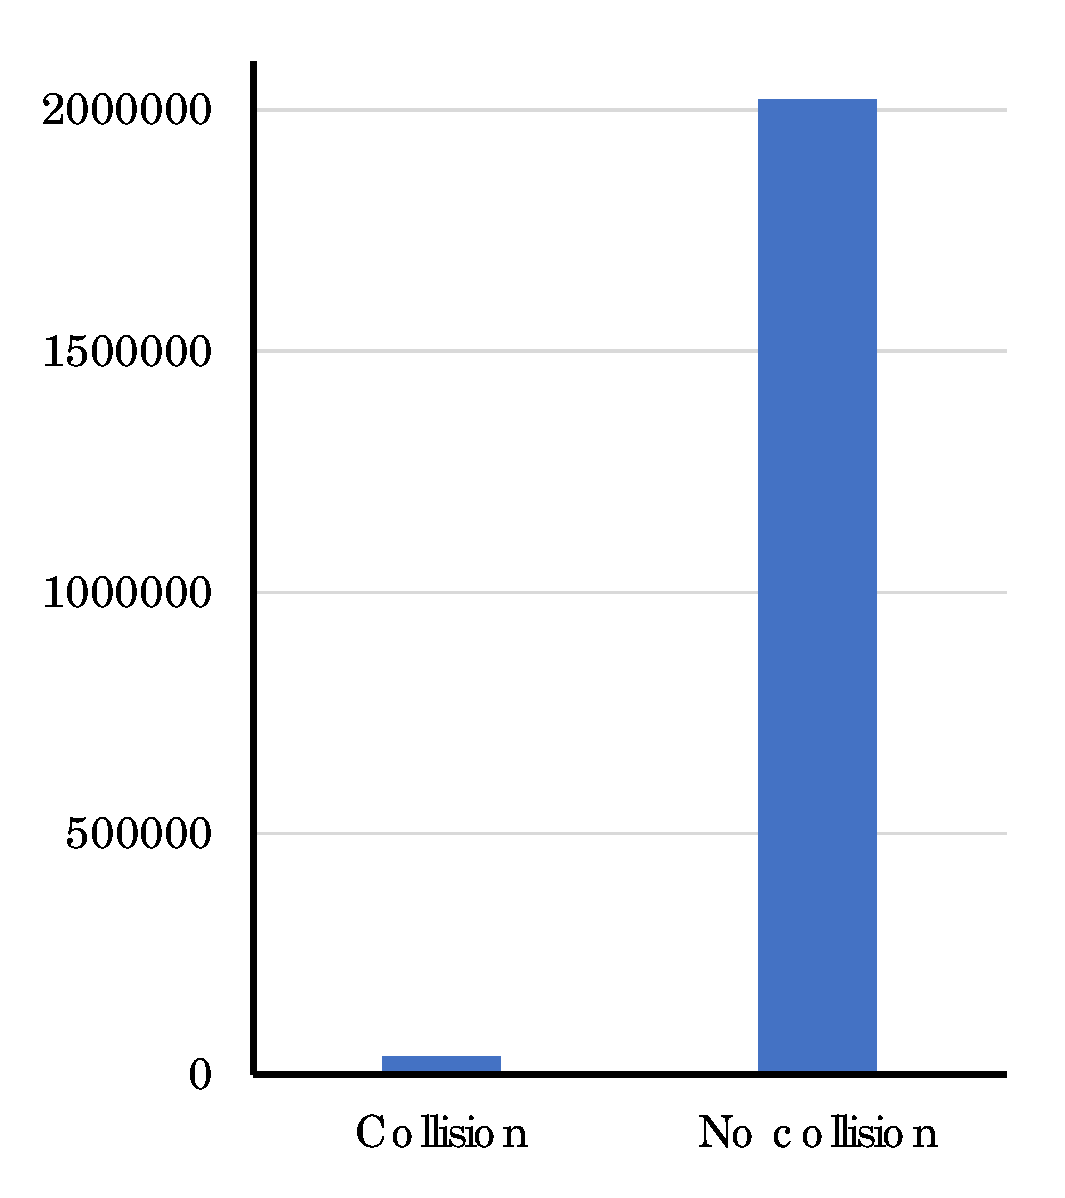
\includegraphics[width=5cm,height=6cm, trim=2cm 4.5cm 2cm 6cm, clip=true]{Data imbalance-cr1}
	\caption{Overview of class balance in the data set.}
	\label{fig:dataimb}
\end{figure}

A statistical predictive model such as logistic regression fitted to such a data set cannot be expected to produce adequate results since the fitting process will be biased toward the majority class, i.e., work orders with no work zone collisions. However, oversampling and under-sampling techniques have been developed to produce a balanced set for training the desired predictive model. In this work, a hybrid method known as synthetic minority oversampling technique (SMOTE), which has been shown to outperform random oversampling and under-sampling method \citep{chawla2002smote} is used to balance the data set. The SMOTE algorithm synthesizes artificial data points close to minority class data by measuring the distance between two points in the minority class and randomly generating a new data point between them. An implementation of the SMOTE algorithm in R programming language is used to balance the training set for model fitting purposes.

%The criteria for determining whether a collision was related to a roadside maintenance work zone was indicated explicitly by the SWITRS data set. However, \cite{fha2018} reports that 77\% of work zone accidents are not identified as such by the police officer at the scene of the collision. Therefore, another collision matching criteria is considered - namely, a collision is identified as a work zone collision if it matches a roadside maintenance work order in location, date, and time for work zones that have a lane closure. This criterion reduces the imbalance of the data set by considering additional work zone collisions, which brings up the total number of work zone accidents from 37,037 to 73,058, or 3.5\% of the data set. The second criterion does not balance the data set; however, it is motivated by its potential ability to compensate for the inaccuracy of work zone collision reporting. For simplification, the first (second) criterion in matching collisions and roadside work zones will be denoted as CR1 (CR2) hereafter.

\section{Method} \label{se:method}
In determining the risk of collision for each roadside maintenance activity based on the features described in Table \ref{tab:features}, a binary classification algorithm capable of evaluating the probability of belonging to a class is the typical method used in literature. For example, \cite{yang2015work} reports that most studies in modeling crashes or work zone injuries use logistic and probit regressions. These regression models are generally more interpretable and can easily inform policy and decision-making processes because they are restricted to only generate a set of limited shapes \citep[][Chapter 2]{james2013introduction}. For example, a logistic regression model can only produce sigmoid shapes, and thus the relationship between the response variable and model features is easy to understand. In contrast, classification methods that generate a wider range of possible shapes for accurate prediction present an interpretability challenge since the effect of an individual feature on the response cannot be understood easily and may not be even consistent. In this analysis, we use two classifiers from the two ends of the interpretability spectrum.

\subsection{Classifiers} \label{sse:classifier}
The logistic regression for determining the probability of a work zone collision is set up according to the following: 
\begin{equation*}
	\ln \frac{p}{1-p} = \beta_0 + \beta_1 x_1 + \ldots + \beta_{J} x_{J},
\end{equation*} where $p$ denotes the probability of work zone collision, $x_j$ for $j=1,\ldots,J$ denotes the predictors listed in Table \ref{tab:features}, and $\beta_j$ are parameters of the model. The logistic regression setup is appropriate for binary classification where, in our case, work zone with and without collision construct the two classes. 
%However, the SWITRS data set also provides a collision severity feature which, for the purposes of this study, is summarized to three ordered classes: work orders with no work zone collisions denoted by CL1, (2) work orders with collisions resulting in property damage denoted by CL2, and (3) work orders with collisions resulting in injuries or fatalities denoted by CL3. The logistic regression framework can be extended to consider ordered classes in different ways: proportional-odds cumulative models, partial proportional-odds cumulative models, adjacent category models, continuous ratio models, and stopping ratio models. However, none of these extensions were able to produce accurate predictions with respect to the defined three classes.

%In addition to these regression methods, which are among the more interpretable classification algorithms,
In addition to logistic regression, which is among the more interpretable classification algorithm, a state-of-the-art technique known as extreme gradient boosting, is also implemented in this work. Extreme gradient boosting (hereafter xgBoost) is an ensemble method for classification and regression trees (CART) where the ensemble of trees is trained via an additive algorithm by optimizing the mean squared error (MSE) as the loss function. For binary classification, this objective function is equivalent to a Taylor expansion of the logistic loss function. Moreover, this technique also implements a regularization term in the objective function measuring the complexity of the fitted trees and penalizing extra branches. This behavior is equivalent to the pruning technique in tree-based models; see \cite{chen2016xgboost}. 
%However, the xgBoost technique cannot handle ordinal response variables in its original form. Therefore, a simple response variable transformation scheme is used to transform the three-class ordinal problem into two binary classification problems. The scheme is described in detail by \cite{frank2001simple} and is shown to perform better than multi-class decision trees such as C4.5 significantly. In this implementation, a binary target variable indicating the severity of the collision is introduced, and the data set is re-labeled according to the following two criteria: The first copy of the data set implements $\mathbbm{1}_{\{\text{target severity}>\text{CL1}\}}$ indicator function to transform its ordinal classes to binary. The second copy applies $\mathbbm{1}_{\{\text{target severity}>\text{CL2}\}}$. Therefore, the probability of each class after training a binary classifier over these two data sets will be:

%\begin{equation*}
%	\begin{aligned}
%		& q_1=1-P(\text{target severity}>\text{CL1}),\\
%		& q_2=P(\text{target severity}>\text{CL1})-P(\text{target severity}>\text{CL2}),\\
%		& q_3=P(\text{target severity}>\text{CL2}).
%	\end{aligned}
%\end{equation*}

\subsection{Feature Selection Models} \label{sse:feature}
Most implementations of logistic %or ordinal 
regression are not able to process non-numeric inputs; therefore, categorical features of Table \ref{tab:features} are transformed into binary dummies by generating, for example, $k - 1$ dummy binary covariates for a variable with $k$ categories. This transformation increases the number of features to 724. To reduce the dimension of the data set, features that have near zero variance or are linearly dependent or highly correlated are removed. This step is necessary because feature selection methods for logistic %and ordinal 
regression models tend to be computationally expensive with large feature sets, and their result is not reliable in assessing the effect a single feature in the presence of collinearity. This is not the case for the xgBoost method as it can easily converge even with large feature sets and the ensemble nature of the algorithm allows it to handle highly correlated features effectively. The data set is then split into training (70\%) and testing (30\%) sets where the SMOTE technique balances only the training set.

To identify major factors contributing to the probability of work zone collision, %and its severity,
two variable selection methods, recursive feature elimination and elastic net, are implemented and compared for logistic regression. Recursive feature elimination proposed by \cite{guyon2002gene} for cancer gene selection is a versatile feature subset selection method that iteratively ranks variables based on their importance to the model accuracy and eliminates the lowest important features. For logistic regression, the importance is equivalent to the standardized coefficient. Therefore, it is crucial to scale the continuous features of Table \ref{tab:features} to a $[0-1]$ range. However, recursive feature elimination is susceptible to selection bias for large feature sets by assigning exaggerated importance to variables that randomly correlate with the response \citep{ambroise2002selection}. This motivates the use of elastic net regularization, which linearly combines two penalty terms of the Ridge and LASSO regressions (least absolute shrinkage and selection operator) and is shown to perform better in a variety of situations when compared to either LASSO or Ridge regressions \citep{zou2005regularization}. Furthermore, it does not present the interpretability issues of the step-wise regression; see \cite{flom2007stopping} and \cite{harrell2015regression}.

Although xgBoost is sometimes used as a feature selection method by considering a cutoff threshold for variable importance, it inherently implements regularization and tree pruning techniques to prevent the boosting process from considering additional features that do not result in considerable objective improvement. These feature elimination measures include a LASSO and Ridge regularization terms and several tree pruning factors such as minimum child weight, which indicates the minimum sum of observation weight in each node before further splits in the tree. However, the xgBoost algorithms does not eliminate a feature from consideration entirely because even when a feature is prevented from being considered for splitting in a particular tree, it might show up in another tree in the boosting process. Thus, the xgBoost algorithm assigns every feature an importance value. However, a selection wrapper algorithm, known as Boruta, originally developed for random forest classifiers, may also be used with the xgBoost technique. This algorithm extends the information by duplicating each feature while shuffling its values. Then, the xgBoost classifier is run again to evaluate feature importance for both the original and `shadow` features. If the importance of an original feature is significantly less than its shadow, the feature is deemed unimportant and rejected. The algorithm stops when no other feature can be rejected \citep{kursa2010feature}.

\subsection{Training and Performance Metrics}\label{sse:training}
%In order to select the best model with the most important factors in estimating the probability of collision (or probability of each severity level), the data set prepared in Section \ref{se:data} should undergo some preprocessing procedures before training. First, the data set described in \ref{tab:features} consists of categorical and continuous variables. Since some of statistical packages in R cannot process categorical variables internally, a 0-1 binary variable for each level of a categorical variable is generated. For example, a variable with $k$ potential levels is replaced with $k-1$ binary variables where $1$ indicates the observed level for a particular data point. Note that this procedure is not necessary for the xgBoost method. This variable transformation increases the feature set to more than 700 features. To reduce the dimension of the feature set and to prepare the data set for logistic \red{and ordinal} regression, linearly dependent variable, highly correlated features $(>=0.75)$, and variables with near zero variances are eliminated from the data set. Since the data set's categorical features are binary, the huge range of some continuous features (e.g., AADT) may cause bias in the model. Therefore, all the continuous variables are scales to a range of $[0-1]$. Finally, the data set is balanced using the SMOTE algorithm (see Section \ref{se:data}) for logistic \red{(and ordinal)} regression.

To select the best subset of features in recursive feature elimination and elastic net methods, the area under the receiver operating characteristic curve (ROC), also known as AUC, is used to evaluate different feature subsets. AUC can be interpreted as the probability of correctly predicting the class of an observation. AUC is selected as the primary performance criterion because of its insensitivity to class imbalance and its invariance with respect to classification probability threshold. In addition to AUC, the Akaike Information Criterion (AIC) for logistic regression is also evaluated and compared between recursive feature elimination and elastic net regression. AIC may be interpreted as a measure of the trade-off between the goodness of fit and complexity of the underlying model \citep{hastie2009elements}.

The primary performance metric for evaluating the contribution of each feature to a boosted tree model is the feature importance, which in the case of the xgBoost algorithm for binary classification, is measured in terms of relative contributions to the minimization of the logistic loss function. However, this measure is reported to be local and inconsistent across models of the same feature set that are trained over different slices of the same data set. This is because feature importance is biased towards lower splits in the classification tree while one expects features responsible for higher splits to be more important. To compensate for this bias, \cite{NIPS2017_7062} introduced another importance measure that compares the contribution of each feature to the overall prediction if the feature took some baseline value. This performance measure is known as Shapley value and is inspired by a game-theoretic approach that determines the payoff for individuals in a coalition with unequal contribution, \cite{shapley1953value}. The advantage of this performance metric is that it can eliminate unimportant features by pushing their importance to zero. 
%The Boruta feature selection algorithm utilizes Shapley importance values to select the most important subset of features.

To eliminate in-sample bias, all the above performance metrics are measured across 10-fold cross-validated sets where the training set is divided into 10 different subsamples. In each iteration of any feature selection model, one of these subsamples is considered to be a testing subsample while the model is trained on the other nine subsamples. This process is repeated for every subsample in each iteration, and thus, the reported performance measures are sample averages over these subsamples. Cross-validated training is also used for parameterization of several xgBoost parameters. The maximum depth of each tree, learning rate, minimum child weight, and the number of iterations are optimized over by a grid search via cross-validated training.

\section{Results} \label{se:results}
This section presents the results of our statistical analyses and identifies major factors that contribute to the risk of collisions at roadside work zones. In fact, we determine that the top four features indicating and contributing to the risk of collision at roadside work zones are: lane closures, work length, historical collision density, and truck AADT.

In particular, Figures \ref{fig:auc}\subref{fig:rfe.auc} and \ref{fig:auc}\subref{fig:net.auc} show the AUC score of the recursive feature elimination and elastic net methods for logistic regression. Both algorithms achieve a similar AUC score, which can be translated to 0.97 probability of correctly classifying an observation. While both feature selection methods achieve good AUC scores, they do not reduce the number of features significantly. Note that after the dimension reduction procedure described in Section \ref{sse:feature}, the total number of features are reduced to 62 from a total of 724. In particular, the recursive feature elimination method only eliminates one feature from consideration when achieving the highest AUC. The elastic net method also behaves similarly. Even considering a pure LASSO regularization, which pushes less important coefficients to zero, results in the selection of 59 features. The AIC score for the best subset identified by the recursive feature elimination is 281187.1, and 282691.8 for elastic net regression. Therefore, considering both AUC and AIC metrics, it seems that recursive feature elimination has performed better than the elastic net regression; however, both methods keep almost all the features and may be susceptible to over-fitting.

\begin{figure}[b!]%
	\centering
	\subfloat[Recursive Feature Elimination]{{\includegraphics[width=7cm, height=5.5cm, trim=1cm 0cm 1cm 0cm, clip=true]{rfe.auc.png}\label{fig:rfe.auc}}}
	\qquad\qquad
	\subfloat[Elastic Net Regression]{{\includegraphics[width=7cm, height=5.5cm, trim=1cm 0cm 1cm 0cm, clip=true]{net.auc.png}\label{fig:net.auc}}}
	\caption{\protect \centering Area under the ROC curve (AUC) for logistic regression.\label{fig:auc}}
\end{figure}

Figure \ref{fig:xgb}\subref{fig:xgb.auc} and \ref{fig:xgb}\subref{fig:xgb.imp} show the overall AUC score and relative contributions of each feature in the xgBoost method. The xgBoost method achieves better AUC scores than the recursive feature elimination and the elastic net regression method at the expense of model complexity. In fact, the xgBoost algorithm in its original form does not eliminate any features and uses all the 724 (dummy) features to predict the test subsamples in the 10-fold cross-validation training. In particular, the features shown in Figure \ref{fig:xgb}\subref{fig:xgb.imp} are only the top 20 most important features according to the xgBoost method.

However, as discussed in Section \ref{sse:feature}, such important features are reported to be inconsistent and local in the literature. This is because the importance of each feature is dependent on its value, and thus may differ if trained on a different slice of the data set. Therefore, to determine a global importance for each feature, Shapley values for boosted trees \citep[developed by][]{NIPS2017_7062} are used to compensate for that effect. As a result, 309 important features are pushed to zero, and thus the dimension of the data set reduces enough for a feasible Boruta implementation. The premis of Boruta algorithm is to test the importance of each feature by shuffling its values and considering the original feature and its shuffled counterpart simultaneously in a model. A feature is confirmed important if its original importance remains significantly greater than its shuffled copy. As a result of 100 Boruta iterations, the number of features is reduced from 411 to 10. In particular, Figure \ref{fig:borutashap}\subref{fig:xgb.boruta} shows the importance of these 10 features in a box and whiskers plot. Features for which the importance of their shuffled copies was not significantly smaller than the original are referred to as `tentative` by the Boruta algorithm. The top four most important features in determining the probability of collision for a roadside maintenance work zone are lane closure, work length, historical collision density, and truck average annual daily traffic.

The effects of feature values on the probability of work zone collision are plotted in Figure \ref{fig:borutashap}\subref{fig:xgb.imp}. In this figure, the horizontal axis measures the impact of the feature value on the outcome of the classifier. The vertical axis shows the 10 features that have been identified as having an impact on a probability of a collision. The effect of the top 4 most important features on the probability of collision is further explored in Section \ref{se:discuss}.

%Figure \ref{fig:borutashap}\subref{fig:xgb.imp} plots the effect of feature values on probability of work zone collision. The horizontal axis measures the impact of the feature value on the outcome of the classifier. In case of the xgBoost method, higher Shapley values correspond to an increase in probability of work zone collision. For example, high values of lane closure in Figure \ref{fig:borutashap}\subref{fig:xgb.imp}, i.e., 1, correspond with higher Shapley values which indicate that having a lane closure increases the probability of work zone collision. The effect of the top 4 most important features on the probability of collision is further explored in Section \ref{se:discuss}.

\begin{figure}[t]%
	\centering
	\subfloat[AUC]{{\includegraphics[width=7cm, height=5.5cm, trim=1cm 0cm 1cm 0cm, clip=true]{xgb.auc.png}\label{fig:xgb.auc}}}
	\qquad\qquad
	\subfloat[Feature Importance]{{\includegraphics[width=7cm, height=5.5cm, trim=1cm 0cm 1cm 0cm, clip=true]{xgb.imp.png}\label{fig:xgb.imp}}}
	\caption{\protect \centering AUC and feature importance for xgBoost.\label{fig:xgb}}
\end{figure}

\begin{figure}[b]%
	\centering
	\subfloat[Boruta Importance]{{\includegraphics[width=7cm, height=5cm, trim=1cm 0cm 1cm 0cm, clip=true]{boruta.imp.png}\label{fig:xgb.boruta}}}
	\qquad\qquad
	\subfloat[Shapley Values]{{\includegraphics[width=7cm, height=5cm, trim=1cm 0cm 1cm 0cm, clip=true]{shap.imp.png}\label{fig:xgb.shap}}}
	\caption{\protect \centering Boruta importance and Shapley values for xgBoost.\label{fig:borutashap}}
\end{figure}

%To identify features contributing to the severity of roadside work zone collisions, two binary classification models are fit according to the discussion in Section \ref{sse:classifier}. Notice that the first binary classification is equivalent to determining the probability of a work zone collision. The second determines the probability of having a work zone collision resulting in injuries or fatalities. The result of this analysis is presented in Appendix \ref{app-severity-res}. It turns out that closure time, and closure length are among the most important factors affecting the severity of roadside work zone collision where longer and lengthier closures increase the probability of having a collision resulting in injury or fatality.

Below, the best fit of the three feature selection models is used to predict the testing data set. The confusion matrices for the recursive feature elimination, elastic net regression, and extreme gradient boosting (xgBoost) are reported in Tables \ref{tab:confusion}\subref{tab:rfe.acc}, \ref{tab:confusion}\subref{tab:net.acc}, and \ref{tab:confusion}\subref{tab:xgb.acc}, respectively. Note that accuracy is evaluated as the rate of true positive and true negative classifications to the total number of observations. Considering the data imbalance discussed in Section \ref{se:data}, a classifier that predicts `no collision` for every observation will predict the correct class more than 98\% of the time. Notice that none of the classifiers in Table \ref{tab:confusion} beat the no information rate. This is typical in highly imbalanced data sets and does not invalidate the interpretation of good performing models such as the xgBoost method. %Note that this problem was the motivation for considering another collision matching criteria, i.e., CR2, in Section \ref{se:data}. %Appendix \ref{app-2ndcriterion-res} presents the results of similar analyses considering collision matching criterion CR2.

\begin{table}
\centering
\subfloat[Recursive feature elimination for logistic regression, Accuracy: 0.828]{
	\begin{tabular}{ccc}
		& \multicolumn{2}{c}{Reference}\\
		\hline
		\multicolumn{1}{c|}{Prediction} 	& No collision 	& Collision\\
		\hline
		\multicolumn{1}{c|}{No collision} 	& 231597		& 1816\\
		\multicolumn{1}{c|}{Collision}		& 46857			& 2721\\
		\hline
	\end{tabular}
	\label{tab:rfe.acc}}
	\qquad\qquad
\subfloat[Elastic net regression for logistic regression, Accuracy: 0.827]{
	\begin{tabular}{ccc}
		& \multicolumn{2}{c}{Reference}\\
		\hline
		\multicolumn{1}{c|}{Prediction} 	& No collision 	& Collision\\
		\hline
		\multicolumn{1}{c|}{No collision} 	& 231464		& 1811\\
		\multicolumn{1}{c|}{Collision}		& 46990			& 2726\\
		\hline
	\end{tabular}
	\label{tab:net.acc}}\\
	%\quad
\subfloat[Extreme gradient boosting for binary classification, Accuracy: 0.911]{
	\begin{tabular}{ccc}
		& \multicolumn{2}{c}{Reference}\\
		\hline
		\multicolumn{1}{c|}{Prediction} 	& No collision 	& Collision\\
		\hline
		\multicolumn{1}{c|}{No collision} 	& 253879		& 699\\
		\multicolumn{1}{c|}{Collision}		& 24575			& 3838\\
		\hline
	\end{tabular}
	\label{tab:xgb.acc}}
	\caption{\protect \centering Confusion matrices for feature selection models.\label{tab:confusion}}
\end{table}

\section{Discussion} \label{se:discuss}
To confirm and assess the results of our classification approach, the top four features identified by the xgBoost algorithm are further explored here. Note that these features were also identified as having a significant effect on the probability of collision in the logistic regression method since their standardized regression coefficients were among the largest. 

In Figure \ref{fig:borutashap}\subref{fig:xgb.boruta}, existence of lane closure is identified as the most important feature in determining the probability of collision for roadside maintenance work zones. Figure \ref{fig:borutashap}\subref{fig:xgb.shap} suggests that roadside work zones with lane closure are exposed to more risk. This result can also be confirmed by Figure \ref{fig:feature.effect}\subref{fig:col.lc}, where the number of collisions in work zones with lane closure is shown to be significantly higher than the number of collisions for roadside work zones without collision between 2013 to 2018. However, one should be careful in interpreting the effect of lane closures on the risk of collision. Our results do not prove that lane closures are responsible for more work zone collisions. Rather, they indicate that maintenance or construction activities which require lane closures are exposed to a higher risk of work zone collision. In fact, upon further exploration, it was found that bridge activities and maintenance activities regarding rigid pavements which typically occur on highway or freeway travel lanes (as opposed to shoulder lanes) have the highest percentage of lane closures. Therefore, lane closures may indicate a higher risk of collision because the underlying work zone for the maintenance or construction activity is set up in travel lanes as opposed to shoulders. 

The next important feature in Figure \ref{fig:borutashap}\subref{fig:xgb.boruta} is work length (in mile). Figure \ref{fig:borutashap}\subref{fig:xgb.shap} does not reveal a stark contrast between short and long work zones; however, it suggests that longer work zones slightly increase the probability of work zone collisions. This is further explored by the violin plot of Figure \ref{fig:feature.effect}\subref{fig:col.wl} where the width of the violin at any particular work length is proportional to the percentage of work orders with or without collision. Figure \ref{fig:feature.effect}\subref{fig:col.wl} clearly shows that longer roadside work zones proportionally correspond with more work zone collisions. It also indicates that maintenance work orders with extremely short or extremely long lengths are expected to incur fewer work zone collisions.

The third important factor, collision density, reveals unexpected results where higher historical collision densities correspond with a reduction in the probability of work zone collision. This is evident in Figure \ref{fig:borutashap}\subref{fig:xgb.shap}. To explore this result further, Figure \ref{fig:feature.effect}\subref{fig:col.cd} depicts the percentage of work orders at any particular collision density by the width of the violin for work zones with and without collisions. According to this figure, higher densities correspond with less work zone collisions when compared to lower collision densities.

Finally, in Figure \ref{fig:feature.effect}\subref{fig:col.ta}, the higher truck AADT values show the highest proportion of work zone collisions. This is in agreement with the results of Figure \ref{fig:borutashap}\subref{fig:xgb.shap}, which suggests that higher values of truck AADT increase the probability of roadside work zone collision. %Appendix \ref{app-severity-res} suggests that in addition to these factors, higher closure times and lengthier lane closures may contribute to the severity of work zone collisions resulting in accidents involving injuries or fatalities.

\begin{figure}[hb!]
	\centering
	\subfloat[Distribution of work zone collisions w.r.t. lane closure]{{\includegraphics[width=7cm, height=5.5cm, trim=1cm 0cm 1cm 0cm, clip=true]{col.lc.png}\label{fig:col.lc}}}
	\qquad\qquad
	\subfloat[Distribution of work zone collisions w.r.t. work length]{{\includegraphics[width=7cm, height=5.5cm, trim=1cm 0cm 1cm 0cm, clip=true]{col.wl.png}\label{fig:col.wl}}}
	\\
	\subfloat[Distribution of work zone collisions w.r.t. collision density]{{\includegraphics[width=7cm, height=5.5cm, trim=1cm 0cm 1cm 0cm, clip=true]{col.cd.png}\label{fig:col.cd}}}
	\qquad\qquad
	\subfloat[Distribution of work zone collisions w.r.t. truck AADT]{{\includegraphics[width=7cm, height=5.5cm, trim=1cm 0cm 1cm 0cm, clip=true]{col.ta.png}\label{fig:col.ta}}}
	\caption{Work zone collisions distribution across the top 4 most important features affecting the probability of work zone collision.}
	\label{fig:feature.effect}
\end{figure}

\subsection{Data Limitations}
No data set is perfect and free of error or missing information. In matching and linking the data sets described in \ref{se:data}, some of the inaccuracies in various Caltrans data sets could not be reconciled except by considering additional assumptions. For example, location data consisting of route ID, county, postmile, or coordinates (latitude and longitude) are used to match work orders with other data sets. However, for some of the collision reports, the only location data consisted of coordinates reported to 4 decimals, which leads to inaccurate coordinates to postmile conversion. Moreover, California postmile system uses multiple prefixes and suffixes to keep track of the ever changing geometry of its roads system but not all their data set stores these prefixes or suffixes when recording work orders and closures. These types of inaccuracies and missing information were compensated for by converting all location data into the best-estimated odometer and allowing a tolerance of 0.25-mile when matching various data sets.

In addition, several features of the SWITRS database (collision reports) such as weather or lighting condition could not be used because the information was not available for any work order that did not correspond with a work zone collision. Furthermore, no information about the injured or fatalities could be inferred since none of the available databases distinguished between Caltrans' workers, passengers, or pedestrian bystanders. Finally, the criteria for determining whether a collision was related to a roadside maintenance work zone was indicated explicitly by the SWITRS data set. However, \cite{fha2018} reports that 77\% of work zone accidents are not identified as such by the police officer at the scene of the collision. 

%Finally, although another collision matching criteria was considered to improve the inaccuracy of police collision reports in indicating a work zone collision, the matching process can only link work orders and collision when the work order was utilizing a lane closures. This is the only case where determining the time of maintenance work orders is possible. As a result, the second collision matching criteria may still underestimate the number of work zone collisions and is susceptible to mis-specification error.

\section{Conclusion} \label{se:conclusion}
In this paper, a data set is developed by combining data from several data bases to provide a more comprehensive description of characteristics of work zone collisions. This enables statistical analyses and classification methods to incorporate more features and derive more accurate results related to factors influencing work zone collisions. We found that lane closures, work length, collision density, and truck  AADT are the most significant factors in determining the probability of collision at the site of roadside maintenance operations. The result of this research can be utilized in decision-making processes when scheduling and planning roadside maintenance or construction works, designing work zones and lane closures, and considering additional safety measures for certain activities. The overall outcome will be improved highway safety for highway workers as well as travelling public.

\section{Acknowledgement} \label{se:acknowledgement}
The work presented in this paper was supported by California Department of Transportation as part of its support of research  at the Advanced Highway Maintenance and Construction Technology (AHMCT) research center at University of California - Davis.


\newpage\clearpage
\bibliographystyle{informs2014}
\bibliography{references}
% Please eliminate the appendix and any references related to it
%\newpage
%\appendix
%\begin{appendices}
%\section{Severity Classification Results}\label{app-severity-res}
%In this section, the results of applying the xgboost learner within a Boruta feature selection model is presented for the $\mathbbm{1}_{\{\text{target severity}>\text{CL2}\}}$ classification problem which classifies work zone collisions with respect to their severity. Note that, as discussed in Section \ref{sse:classifier}, this classifier may be combined with the results of the original classification model to replicate an ordinal classification where class probabilities are ordered as $p(\text{collision with injuries or fatalities}) \leq p(\text{collision with property damage only}) \leq p(\text{no collision})$. The Boruta feature selection method confirms 10 features in this case and rejects all other features as unimportant. Figure \ref{fig:borutashap-ordered}\subref{fig:xgb.boruta.ordered} shows that in contrast to the original model, closure time, facility, and closure length are the top most important features in classifying collisions that resulted in injury or fatality. Figure \ref{fig:borutashap-ordered}\subref{fig:xgb.shap.ordered} shows that longer closure times and lengthier lane closures increase the probability of having a work zone collision resulting in injury or fatality. However, the Shapley values for work orders with closures on freeways do not agree with Boruta results because they concentrated around 0 which means that they do not move the probability of severe collisions by much. These results can be confirmed by further exploring the data sets
%with respect to the new identified features: closure time, closure facility, and closure length.

%begin{figure}[h]%
%	\centering
%	\subfloat[Boruta Importance]{{\includegraphics[width=7cm, height=5cm, trim=1cm 0cm 1cm 0cm, clip=true]{boruta.imp.ordered.png}\label{fig:xgb.boruta.ordered}}}
%	\qquad\qquad
%	\subfloat[Shapley Values]{{\includegraphics[width=7cm, height=5cm, trim=1cm 0cm 1cm 0cm, clip=true]{shap.imp.ordered.png}\label{fig:xgb.shap.ordered}}}
%	\caption{\protect \centering Boruta importance and Shapley values for xgBoost.\label{fig:borutashap-ordered}}
%\end{figure}

%Figure \ref{fig:feature.effect.oredered} further explores the relationship between collisions resulting in injury or fatality and closure length, closure facility, and closure time. In particular, Figure \ref{fig:feature.effect.oredered}\subref{fig:col.ct.ordered} shows that longer closure times increase the probability of severe collisions slightly. Figure \ref{fig:feature.effect.oredered}\subref{fig:col.fc.ordered} confirms that lane closures on freeways is not significantly riskier than other facilities such as high-occupancy vehicle lanes. Finally, Figure \ref{fig:feature.effect}\subref{fig:col.cl.ordered} shows that lengthier lane closures correspond with more severe collisions proportionally.

%\begin{figure}[t]
%	\centering
%	\subfloat[Distribution of work zone collisions w.r.t. closure time]{{\includegraphics[width=7cm, height=5.5cm, trim=1cm 0cm 1cm 0cm, clip=true]{col.ct.ordered.png}\label{fig:col.ct.ordered}}}
%	\qquad\qquad
%	\subfloat[Distribution of work zone collisions w.r.t. closure facility]{{\includegraphics[width=7cm, height=5.5cm, trim=1cm 0cm 1cm 0cm, clip=true]{col.fc.ordered.png}\label{fig:col.fc.ordered}}}
%	\\
%	\subfloat[Distribution of work zone collisions w.r.t. closure length]{{\includegraphics[width=7cm, height=5.5cm, trim=1cm 0cm 1cm 0cm, clip=true]{col.cl.ordered.png}\label{fig:col.cl.ordered}}}
%	\caption{Distribution of work zone collisions resulting in injury or fatality across the top 3 most important feature.}
%	\label{fig:feature.effect.oredered}
%\end{figure} 

%\section{Second Collision Matching Criterion}\label{app-2ndcriterion-res}
%The main paper's results are produced by training the classification model on a data set in which roadside maintenance work orders are matched with collisions only when the collision report explicitly identifies a work/construction zone as the scene of a collision. Recall from Section \ref{se:data} that this is not always accurate and it is estimated that as much as 77\% of work zone collisions are not reported as such in collision reports \citep{fha2018}. Therefore, another collision matching criterion, CR2, is motivated which is described in Section \ref{se:data}. Here, we present the results of implementing an extreme gradient boosting within Boruta feature selection wrapper and analyze its feature importances using Shapley values. In particular, Figure \ref{fig:borutashap-cr2}\subref{fig:xgb.boruta.cr2} identifies the most important features in classifying a roadside maintenance work order with respect to the probability of collision. Figure \ref{fig:borutashap-cr2}\subref{fig:xgb.shap.cr2} shows how each feature values affect the probability of work zone collision. However, these results may not be as reliable as the original data set since the rate of false positive to true positive for this classification problem is slightly bigger than one which means that the classification algorithm is not to distinguish between roadside maintenance work orders that resulted in collision and those without a work zone collision.

%\begin{figure}[h]%
%	\centering
%	\subfloat[Boruta Importance]{{\includegraphics[width=7cm, height=5cm, trim=1cm 0cm 1cm 0cm, clip=true]{boruta.imp.2ndcr.png}\label{fig:xgb.boruta.cr2}}}
%	\qquad\qquad
%	\subfloat[Shapley Values]{{\includegraphics[width=7cm, height=5cm, trim=1cm 0cm 1cm 0cm, clip=true]{shap.imp.2ndcr.png}\label{fig:xgb.shap.cr2}}}
%	\caption{\protect \centering Boruta importance and Shapley values considering CR2\label{fig:borutashap-cr2}}
%\end{figure}

%\end{appendices}
\end{document}